\chapter{Office 365 Education A1 の利用開始手続き}\label{cap:M365A1}

Windows 10 デバイスを Intune で管理するためには、Azure Active Directory へデバイスを登録する仕組みを事前に作っておく必要がございます。第\ref{cap:M365A1}では、その準備のために教育機関向けに無償で提供されている Office 365 Education A1 を利用開始するための手続きに関して解説いたします。

%%%%%%%%%%%%%%%%%%%%%%%%%%%%%%%%%%%%%%%%%%%%%%%%%%%%%%%%%%%%%%%%%%%%%%%%%%%%%%%%
\section{Office 365 Educaiton A1 の利用開始手続きの流れ}
%%%%%%%%%%%%%%%%%%%%%%%%%%%%%%%%%%%%%%%%%%%%%%%%%%%%%%%%%%%%%%%%%%%%%%%%%%%%%%%%

Office 365 Education A1 の利用開始までの手続きを図\ref{fig:O365A1}に示します。では順番に解説していきたいと思います。

\begin{figure}[h]
    \centering
    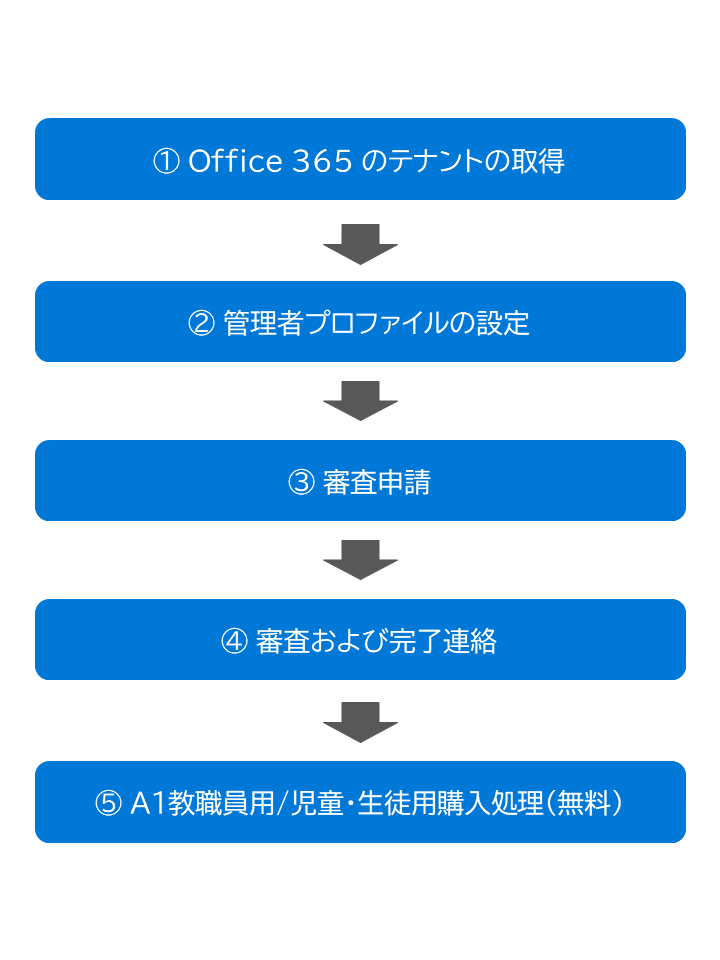
\includegraphics[width=7cm]{figures/O365A1.png}
    \caption{Office 365 Education A1の手続きの流れ}
    \label{fig:O365A1}
\end{figure}

\newpage 

%%%%%%%%%%%%%%%%%%%%%%%%%%%%%%%%%%%%%%%%%%%%%%%%%%%%%%%%%%%%%%%%%%%%%%%%%%%%%%%%
\begin{figure*}[h]
    \begin{minipage}{1.0\textwidth}
        \section{Office 365のテナントの取得}
        \label{sec:Office365テナント取得}
            まずはじめにOffice 365のテナントを取得します。すでに Office 365 Education のテナントを所有している場合には、本手続きは不要です。
    \end{minipage}
\end{figure*}
%%%%%%%%%%%%%%%%%%%%%%%%%%%%%%%%%%%%%%%%%%%%%%%%%%%%%%%%%%%%%%%%%%%%%%%%%%%%%%%%

\begin{figure*}[h]
    \begin{minipage}{0.6\textwidth}
        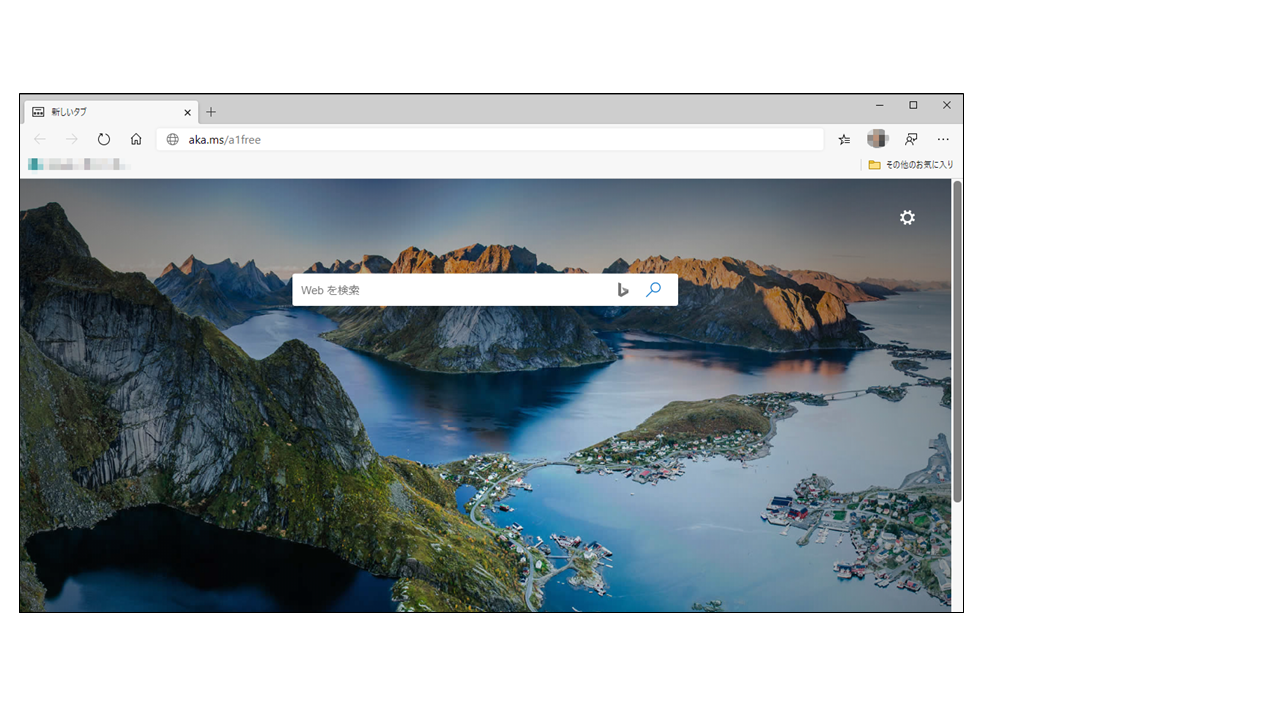
\includegraphics[width=12cm]{figures/O365A1_submission00.png}
    \end{minipage}
    \begin{minipage}{0.4\textwidth}
        Webブラウザから、\url{https://aka.ms/a1free} にアクセスします。
    \end{minipage}
\end{figure*}


\begin{figure*}[h]
    \begin{minipage}{0.6\textwidth}
        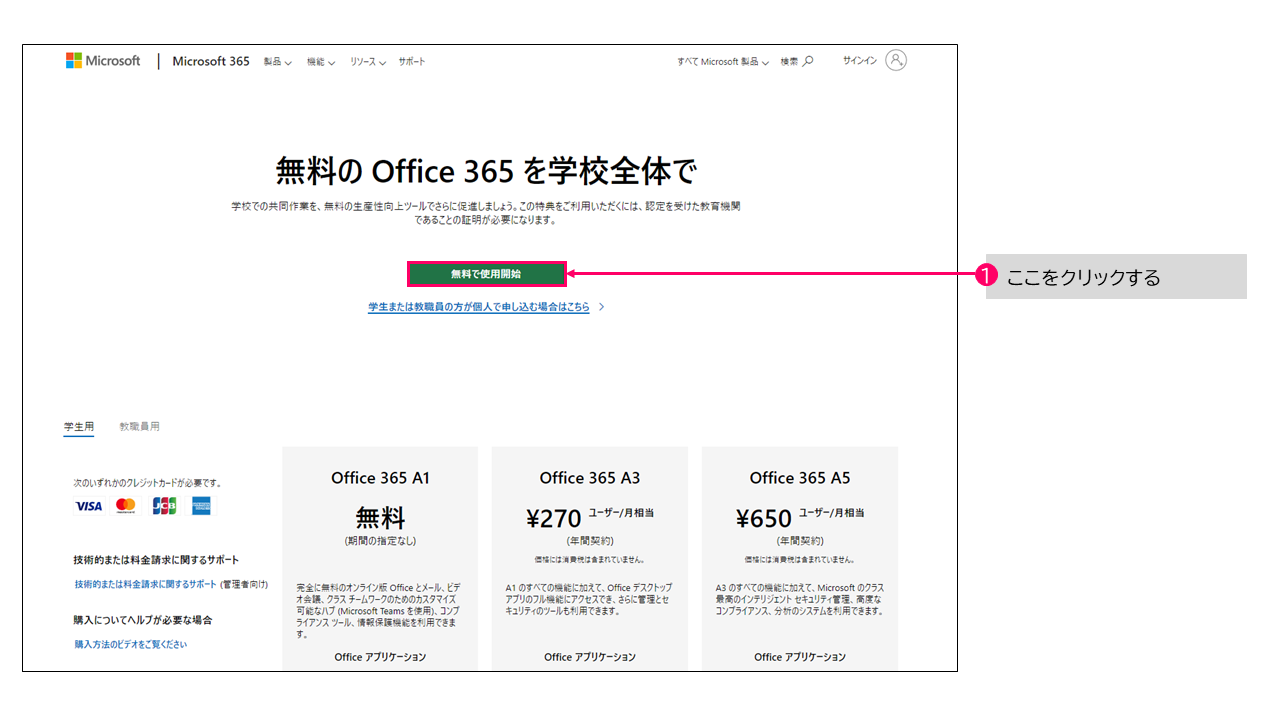
\includegraphics[width=10cm]{figures/O365A1_submission01.png}
    \end{minipage}
    \begin{minipage}{0.4\textwidth}
        \textbf{「Office 365 を学校全体で」}の画面が表示されたら、\textbf{【無料で開始する】}をクリックします。
    \end{minipage}
\end{figure*}

\begin{figure*}[h]
    \begin{minipage}{0.6\textwidth}
        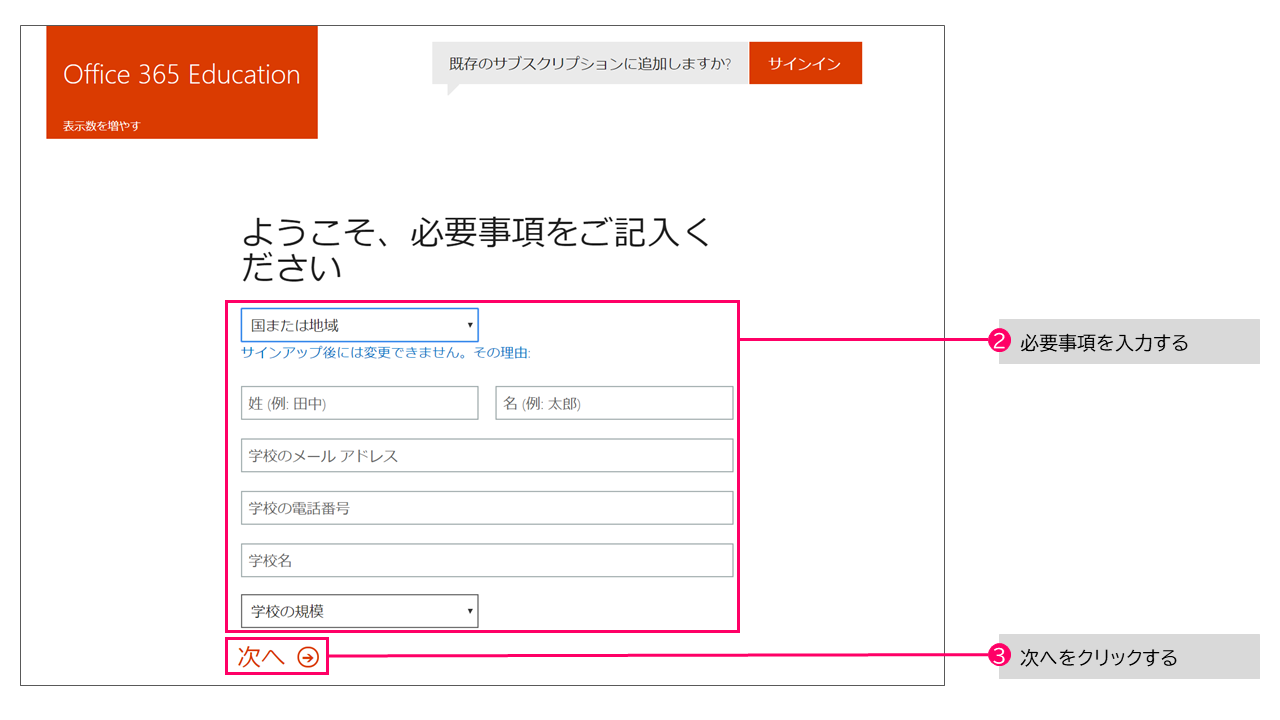
\includegraphics[width=10cm]{figures/O365A1_submission02.png}
    \end{minipage}
    \begin{minipage}{0.4\textwidth}
       \textbf{「ようこそ、必要事項をご記入ください」}の画面が表示されたら、国、氏名、学校のメールアドレス、学校の電話番号、学校名、学校の規模を入力し、\textbf{【次へ】}をクリックします。
    \end{minipage}
\end{figure*}

\begin{figure*}[h]
    \begin{minipage}{0.6\textwidth}
        \hspace{-1.2cm}
        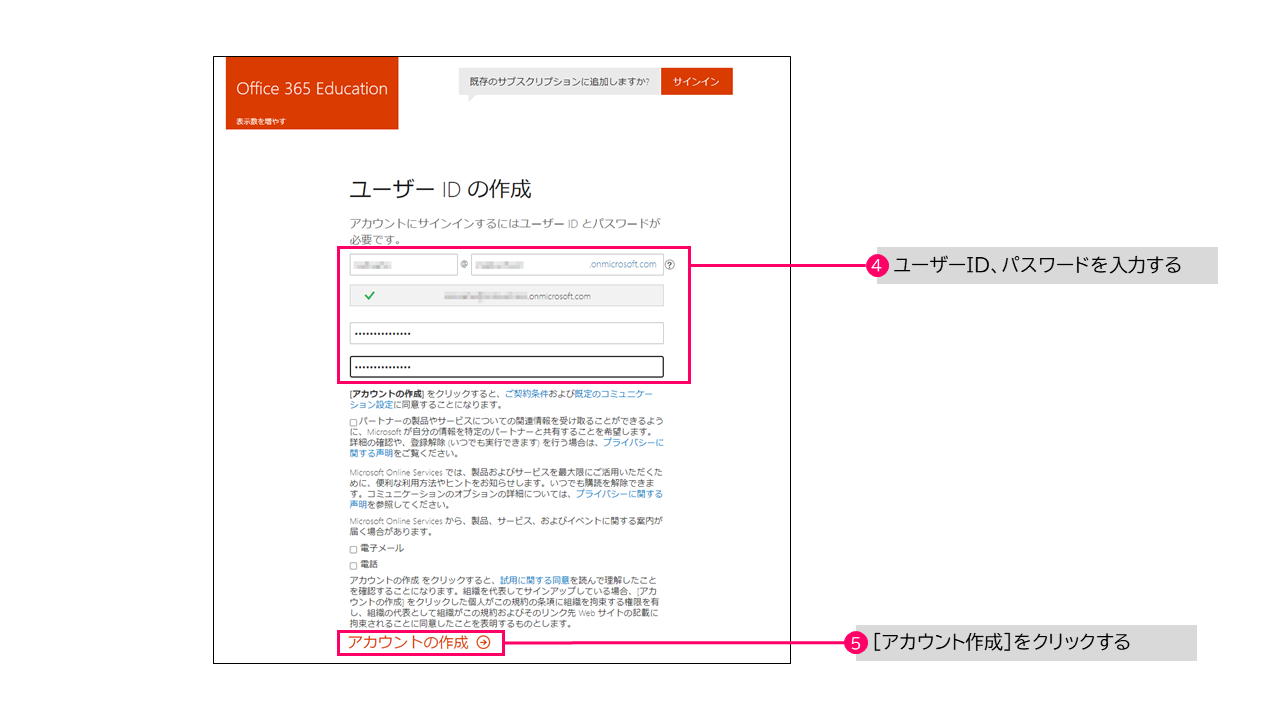
\includegraphics[width=11cm]{figures/O365A1_submission03.png}
    \end{minipage}
    \begin{minipage}{0.4\textwidth}
       \textbf{「ユーザーIDの作成」}の画面が表示されたら、ユーザーID、パスワードを入力し、\textbf{【アカウントの作成】}をクリックします。
    \end{minipage}
\end{figure*}

\begin{figure*}[h]
    \begin{minipage}{0.6\textwidth}
        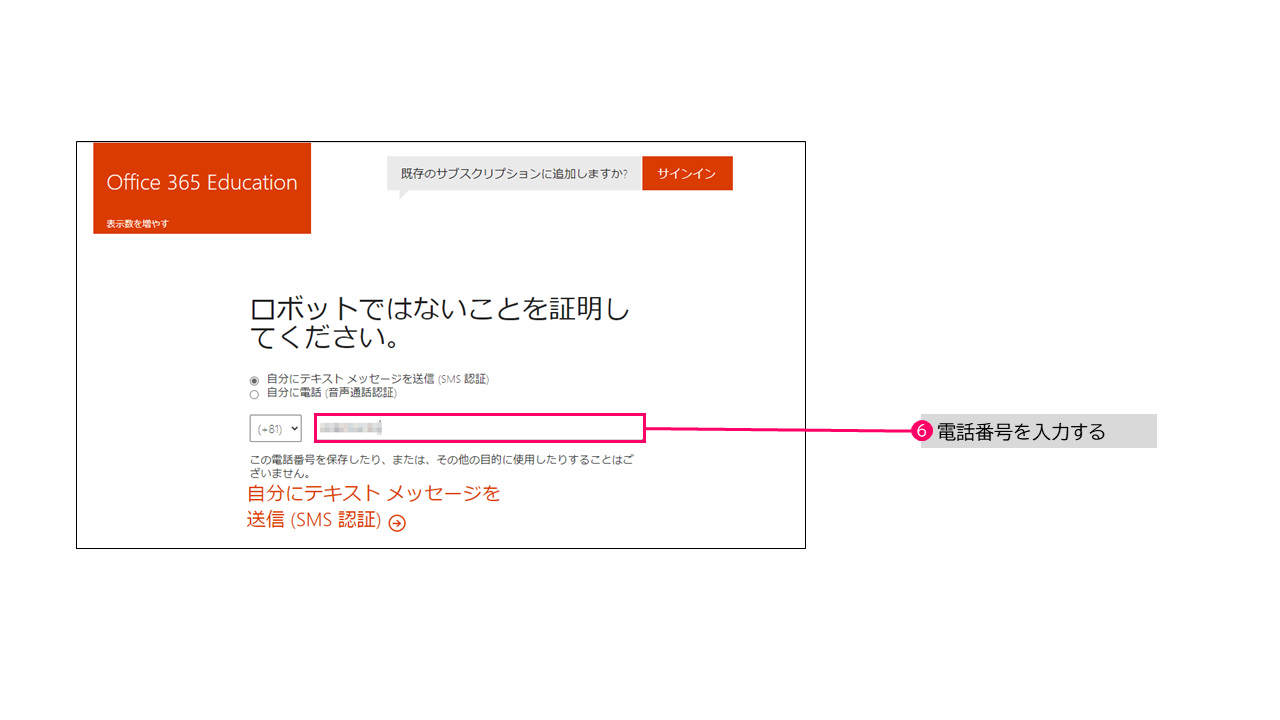
\includegraphics[width=10cm]{figures/O365A1_submission04.png}
    \end{minipage}
    \begin{minipage}{0.4\textwidth}
       \textbf{「ロボットでないことを証明してください」}の画面が表示されたら、テキストメッセージ(SMS)を受けて取れる携帯電話の電話番号を入力し、\textbf{【自分にテキストメッセージを送信(SMS認証)】}をクリックします。
    \end{minipage}
\end{figure*}

\begin{figure*}[h]
    \begin{minipage}{0.6\textwidth}
        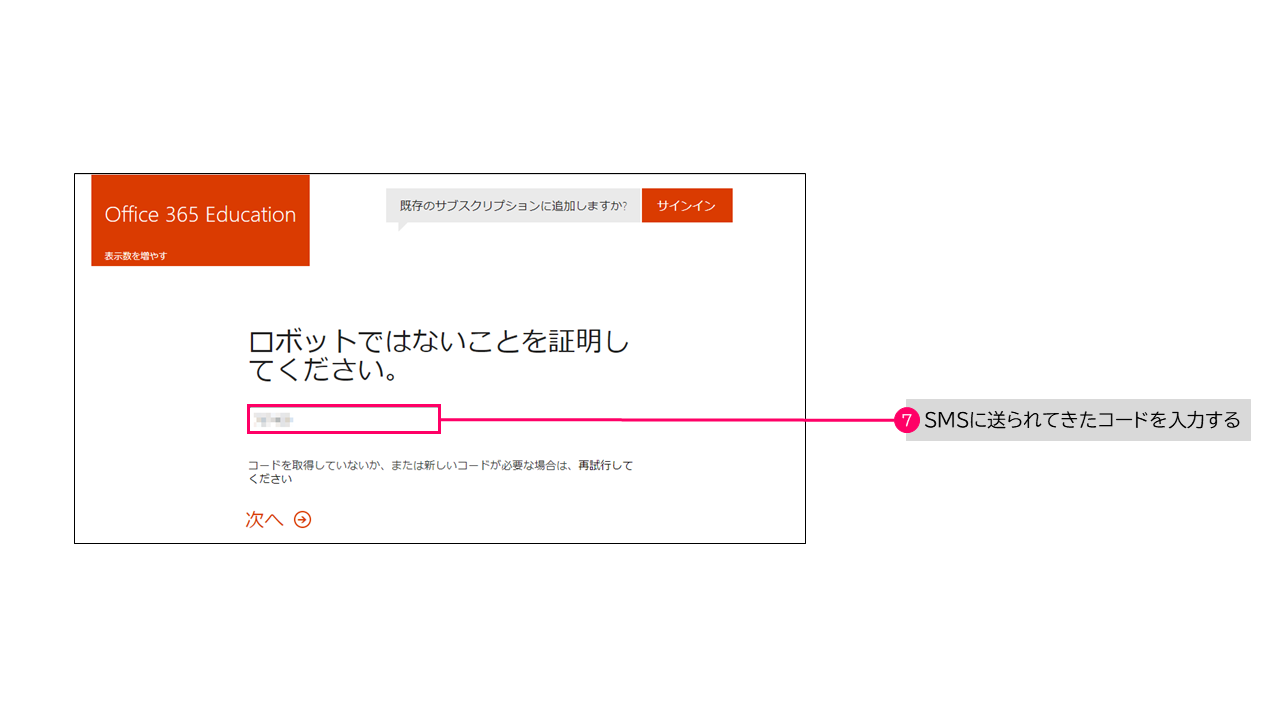
\includegraphics[width=10cm]{figures/O365A1_submission05.png}
    \end{minipage}
    \begin{minipage}{0.4\textwidth}
       携帯電話に、テキストメッセージ(SMS)が送られてきた番号を入力し、\textbf{【次へ】}をクリックします。
    \end{minipage}
\end{figure*}

\begin{figure*}[h]
    \begin{minipage}{0.6\textwidth}
        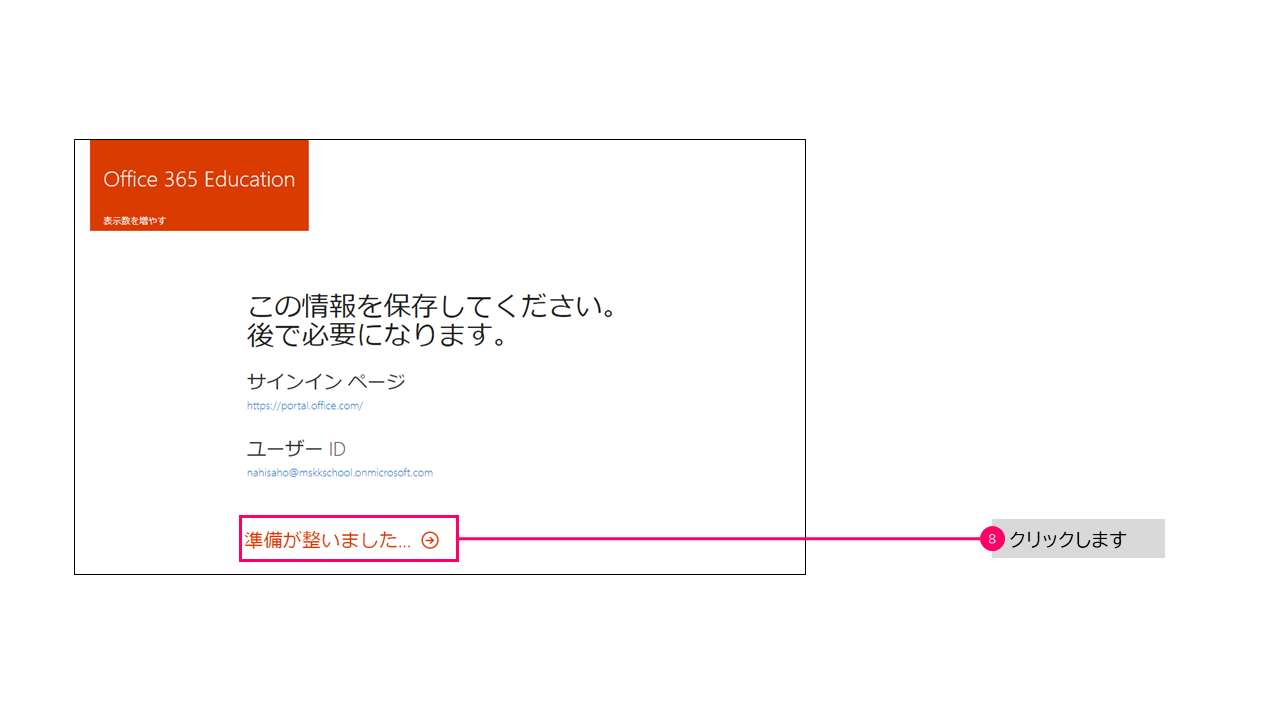
\includegraphics[width=10cm]{figures/O365A1_submission06.png}
    \end{minipage}
    \begin{minipage}{0.4\textwidth}
       \textbf{「この情報を保存してください。後で必要になります」}の画面が表示されたら、\textbf{【準備が整いました】}をクリックします。
    \end{minipage}
\end{figure*}

\begin{figure*}[h]
    \begin{minipage}{0.6\textwidth}
        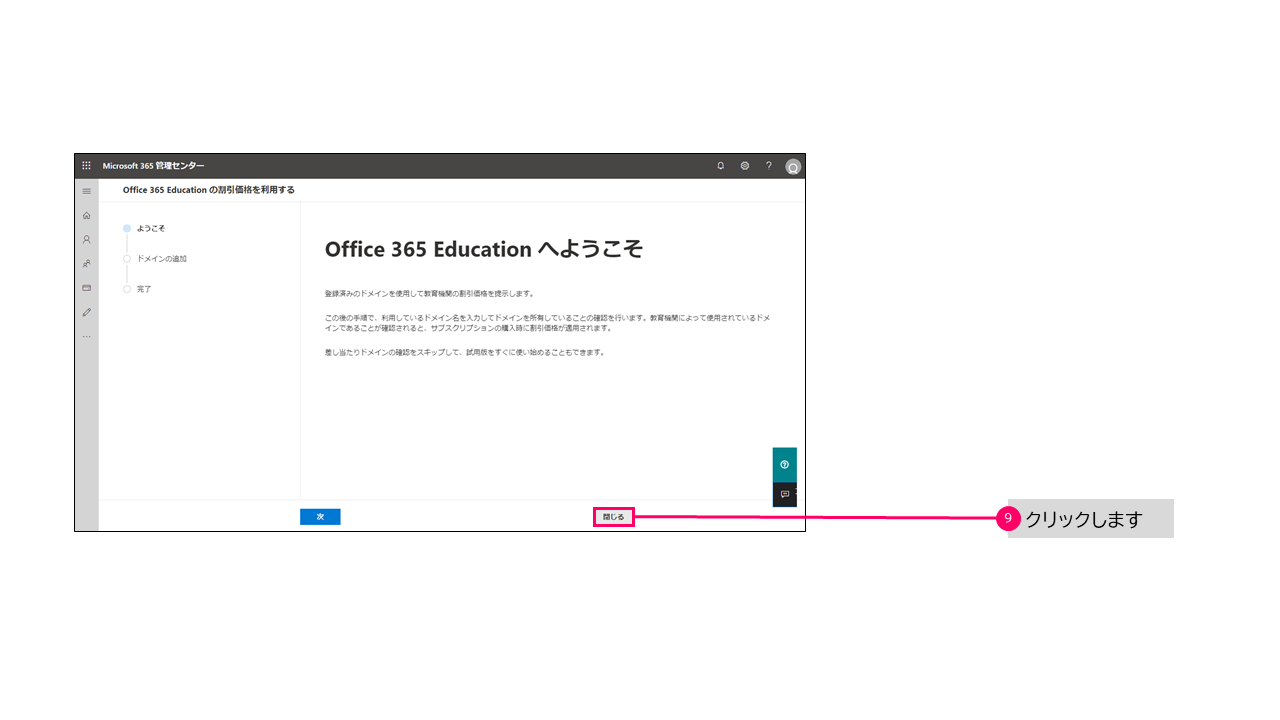
\includegraphics[width=10cm]{figures/O365A1_submission07.png}
    \end{minipage}
    \begin{minipage}{0.4\textwidth}
       \textbf{「Office 365 へようこそ」}の画面が表示されたら、\textbf{【閉じる】}をクリックします。
    \end{minipage}
\end{figure*}

\begin{figure*}[h]
    \begin{minipage}{1.0\textwidth}
        ここまでの作業で作業で、Office 365 Education A1 のテナントが作成されました。この状態では6ヶ月の試用版を利用している状況ですので、Office 365 Education A1 を正式に利用するための手続きをしていきます。
    \end{minipage}
    \vspace{3cm}
\end{figure*}


%%%%%%%%%%%%%%%%%%%%%%%%%%%%%%%%%%%%%%%%%%%%%%%%%%%%%%%%%%%%%%%%%%%%%%%%%%%%%%%%
\begin{figure*}[h]
    \begin{minipage}{1.0\textwidth}
        \section{管理者プロファイルの設定}
        ここでは、Office 365 Education A1 の手続きに必要な管理者プロファイルの登録方法に関して解説いたします。
    \end{minipage}
\end{figure*}
%%%%%%%%%%%%%%%%%%%%%%%%%%%%%%%%%%%%%%%%%%%%%%%%%%%%%%%%%%%%%%%%%%%%%%%%%%%%%%%%

\begin{figure*}[h]
    \begin{minipage}{0.6\textwidth}
        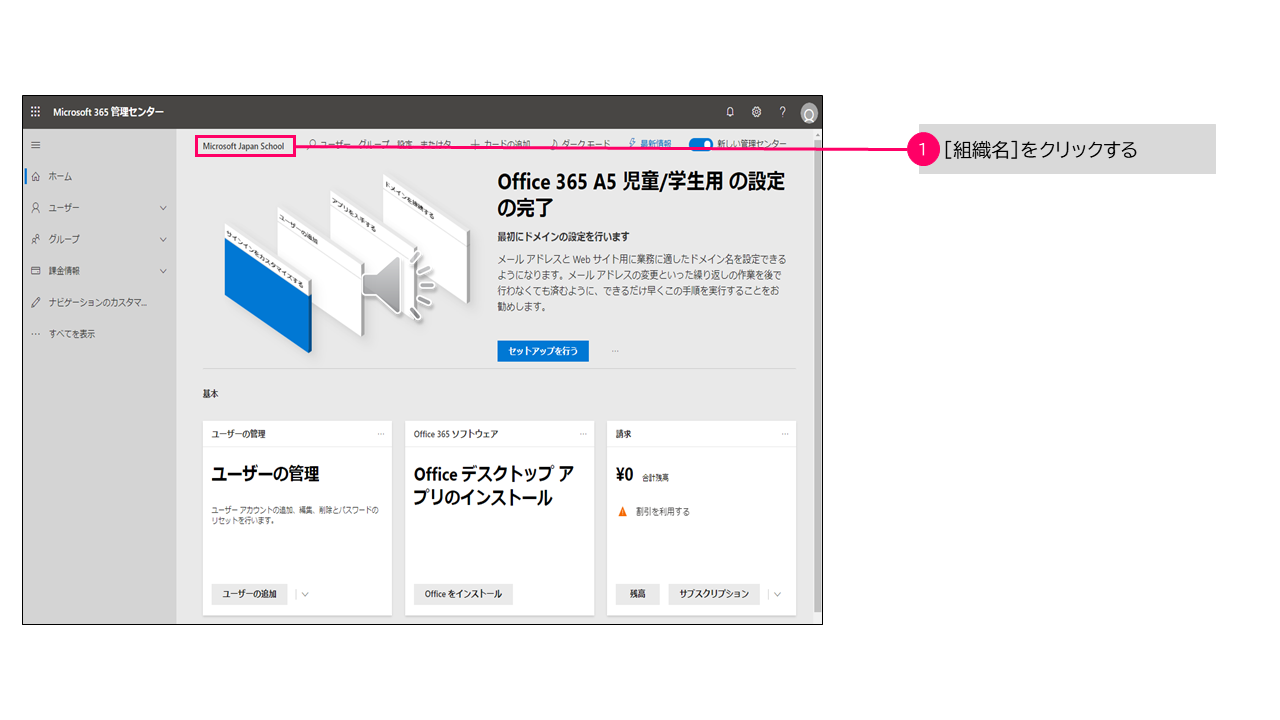
\includegraphics[width=10cm]{figures/O365A1_profile00.png}
    \end{minipage}
    \begin{minipage}{0.4\textwidth}
       画面左上の\textbf{【組織(学校)名】}をクリックします。
    \end{minipage}
\end{figure*}

\begin{figure*}[h]
    \begin{minipage}{0.6\textwidth}
        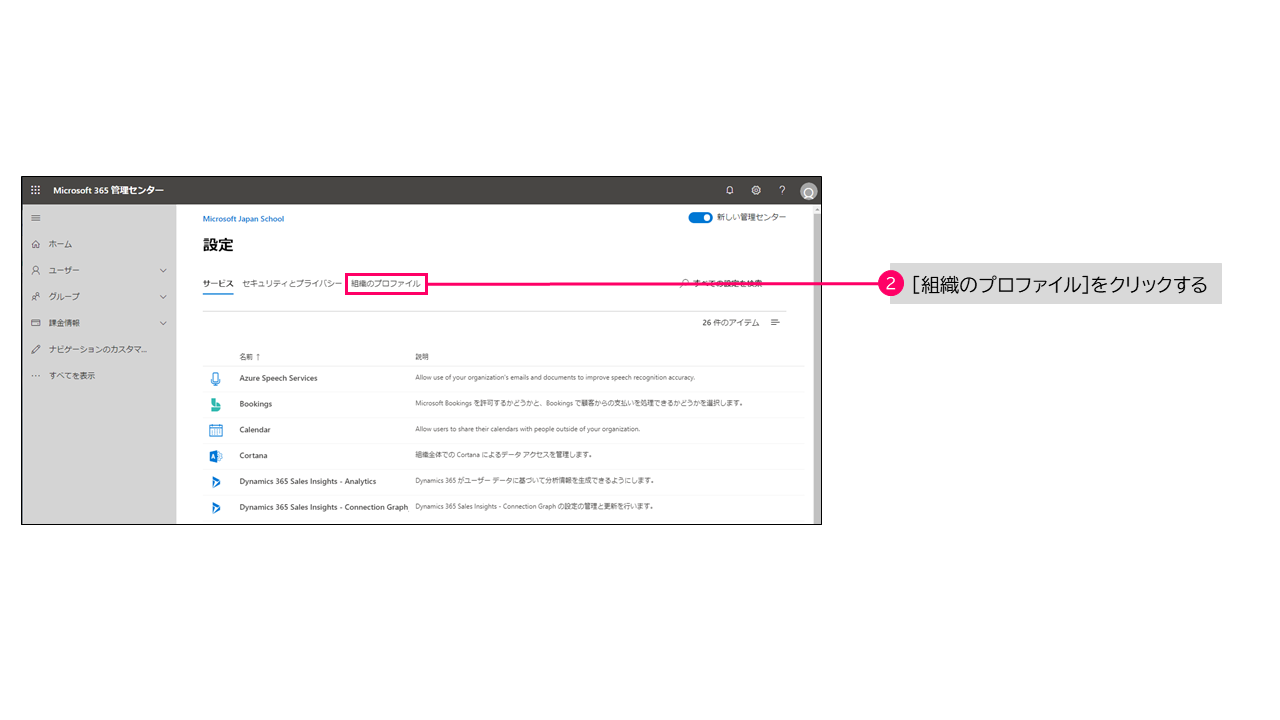
\includegraphics[width=10cm]{figures/O365A1_profile01.png}
    \end{minipage}
    \begin{minipage}{0.4\textwidth}
       \textbf{「設定」}が表示されたら\textbf{【組織のプロファイル】}をクリックします。
    \end{minipage}
\end{figure*}

\begin{figure*}[h]
    \begin{minipage}{0.6\textwidth}
        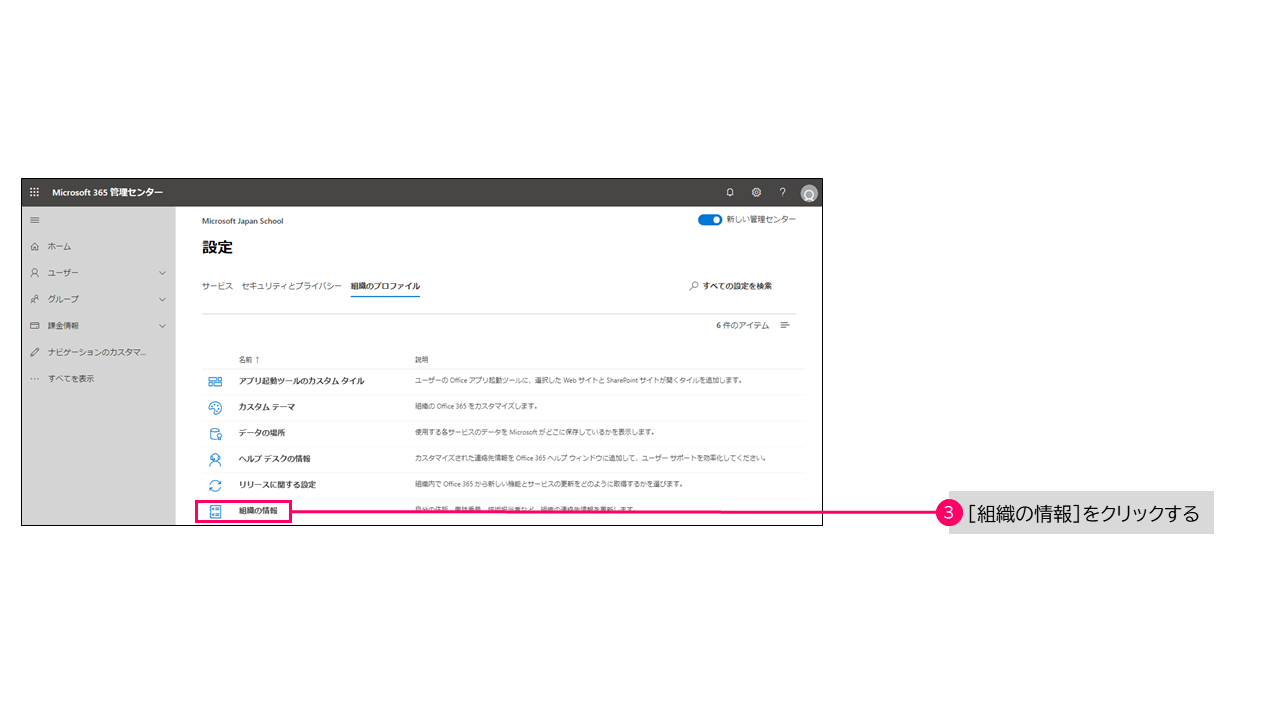
\includegraphics[width=10cm]{figures/O365A1_profile02.png}
    \end{minipage}
    \begin{minipage}{0.4\textwidth}
       次に\textbf{【組織の情報】}をクリックします。
    \end{minipage}
\end{figure*}

\begin{figure*}[h]
    \begin{minipage}{0.6\textwidth}
        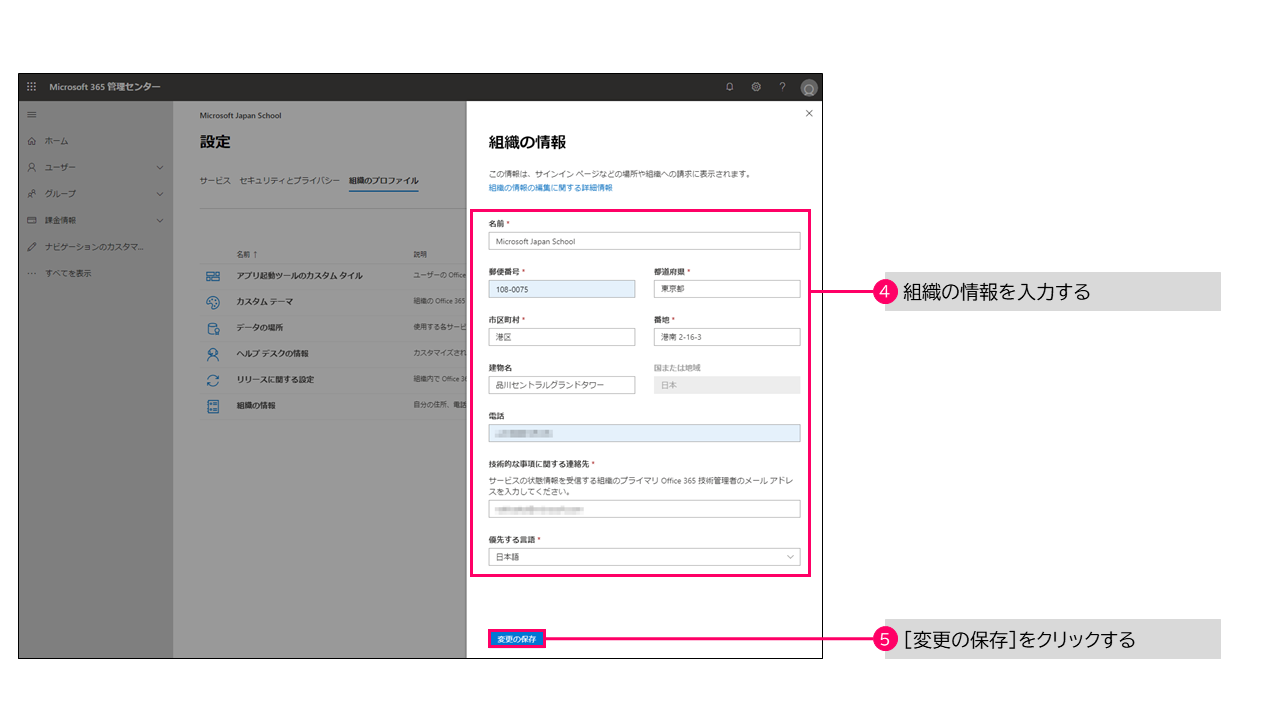
\includegraphics[width=10cm]{figures/O365A1_profile03.png}
    \end{minipage}
    \begin{minipage}{0.4\textwidth}
       \textbf{「組織の情報」}を入力し、\textbf{【変更を保存】}をクリックします。
    \end{minipage}
\end{figure*}

%%%%%%%%%%%%%%%%%%%%%%%%%%%%%%%%%%%%%%%%%%%%%%%%%%%%%%%%%%%%%%%%%%%%%%%%%%%%%%%%
\begin{figure*}[h]
    \begin{minipage}{1.0\textwidth}
        \section{審査申請}
        \label{sec:審査申請}
        Office 365 Education A1 を継続的に利用するには、教育機関としての審査が必要となります。また、追加でライセンスを取得したい場合にも、審査請求と同じ方法で追加申請することが可能です。ここではでは、審査申請の方法について解説いたします。
    \end{minipage}
\end{figure*}
%%%%%%%%%%%%%%%%%%%%%%%%%%%%%%%%%%%%%%%%%%%%%%%%%%%%%%%%%%%%%%%%%%%%%%%%%%%%%%%%

\begin{figure*}[h]
    \begin{minipage}{0.6\textwidth}
        \vspace{-2cm}
        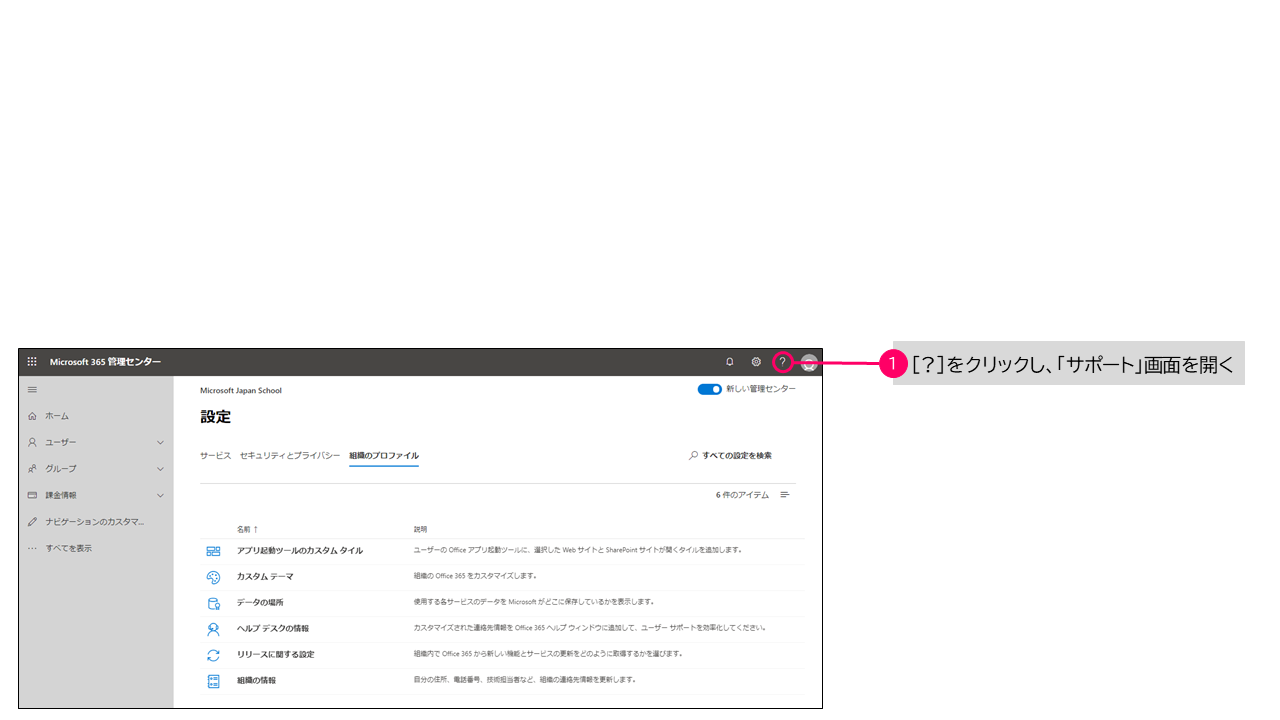
\includegraphics[width=10cm]{figures/O365A1_request00.png}
    \end{minipage}
    \begin{minipage}{0.4\textwidth}
       審査手続きを行うためにサポートへ問い合わせを行います。まずはじめに画面右上の\textbf{【?】}をクリックします。
    \end{minipage}
\end{figure*}

\begin{figure*}[h]
    \begin{minipage}{0.6\textwidth}
        \vspace{-1cm}
        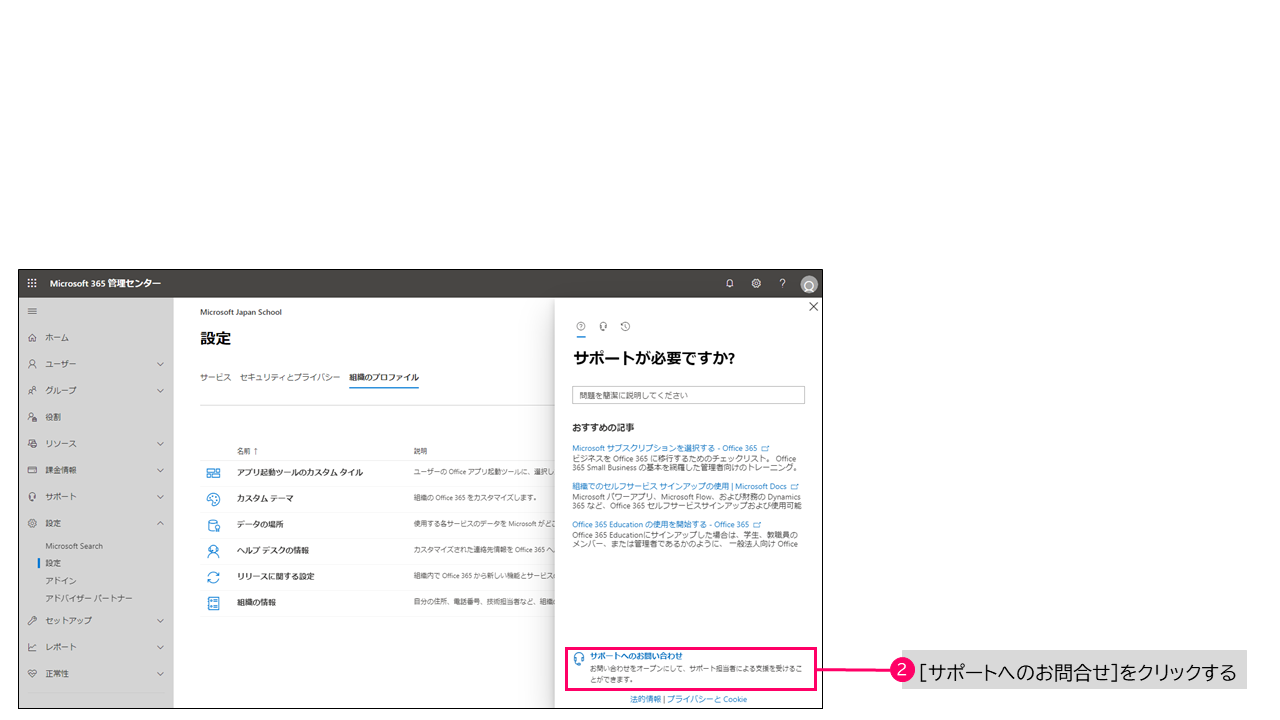
\includegraphics[width=10cm]{figures/O365A1_request01.png}
    \end{minipage}
    \begin{minipage}{0.4\textwidth}
       \textbf{「サポートが必要ですか?」}の画面が開いたら、\textbf{【サポートへのお問合せ】}をクリックします。
    \end{minipage}
\end{figure*}

\begin{figure*}[h]
    \begin{minipage}{0.6\textwidth}
        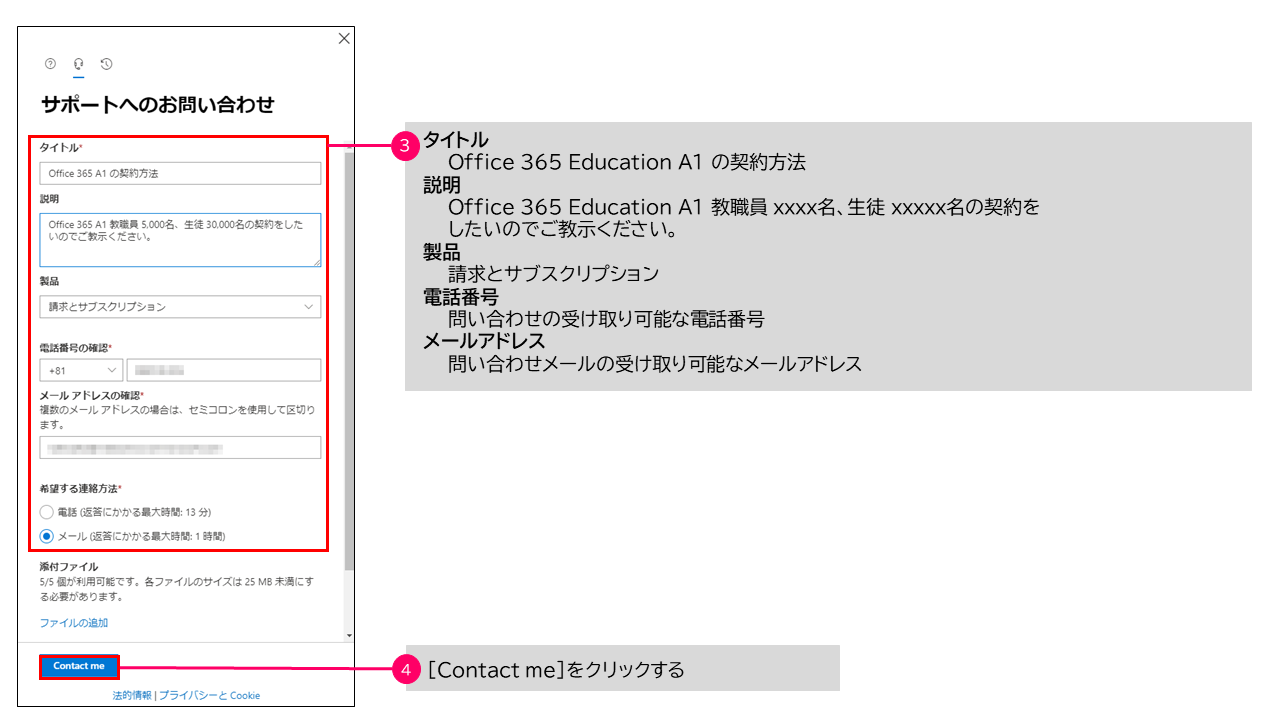
\includegraphics[width=10cm]{figures/O365A1_request02.png}
    \end{minipage}
    \begin{minipage}{0.4\textwidth}
       \textbf{「サポートへのお問合せ」}の画面が開いたら、タイトルに\textbf{「Office 365 Education A1 の契約方法」}、説明に\textbf{「Office 365 Education A1 教職員 xxxx名、生徒 xxxx名の契約をしたいのでご教示ください。}、製品に\textbf{「請求とサブスクリプション」}、電話番号に\textbf{「問い合わせかの受け取り可能な電話番号」}、メールアドレスに\textbf{「問い合わせメールの受け取り可能なメールアドレス」}を入力し、\textbf{【Contact me】}をクリックします。
    \end{minipage}
\end{figure*}


%%%%%%%%%%%%%%%%%%%%%%%%%%%%%%%%%%%%%%%%%%%%%%%%%%%%%%%%%%%%%%%%%%%%%%%%%%%%%%%%
\begin{figure*}[t]
    \begin{minipage}{1.0\textwidth}
        \section{審査および完了連絡}
        \label{sec:Office365審査}
            審査は以下の手順で実施されます。
    \end{minipage}
\end{figure*}
%%%%%%%%%%%%%%%%%%%%%%%%%%%%%%%%%%%%%%%%%%%%%%%%%%%%%%%%%%%%%%%%%%%%%%%%%%%%%%%%

\begin{figure*}[h]
    \centering
    \vspace{-6cm}
    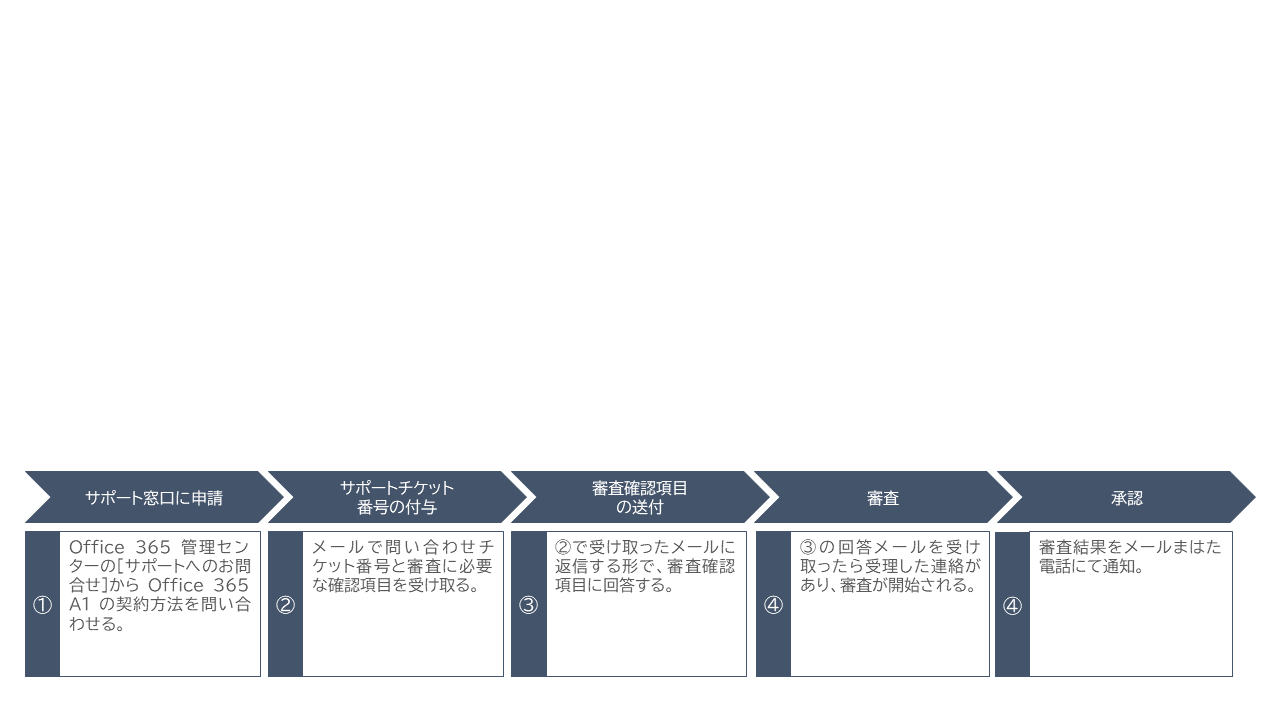
\includegraphics[width=17cm]{figures/O365A1_review00.png}
    \caption{審査の手順}
    \label{fig:審査の手順}
\end{figure*}

\begin{figure*}[h]
    \begin{minipage}{1.0\textwidth}
        審査確認項目(下記はあくまで参考例です。審査確認項目は変更される可能性がございます。)
    \end{minipage}
\end{figure*}


\begin{figure*}[h]
    \centering
    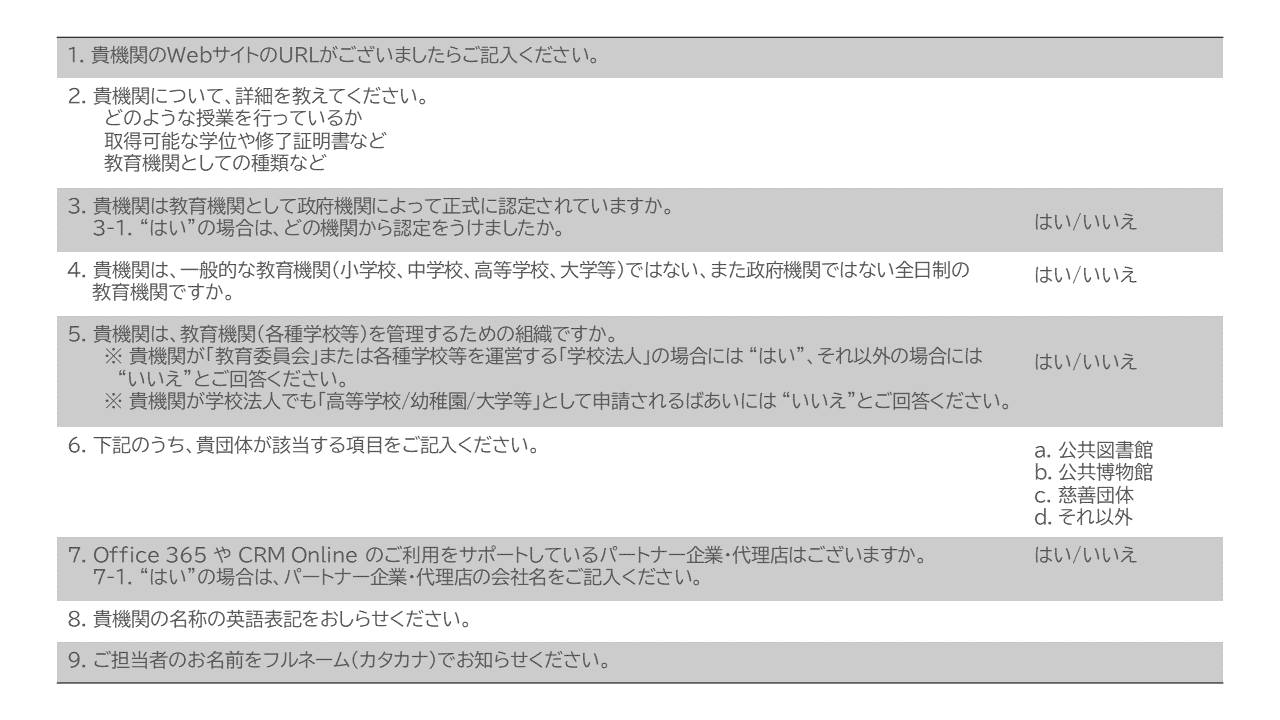
\includegraphics[width=17cm]{figures/O365A1_review01.png}
    \vspace{5cm}
\end{figure*}

%%%%%%%%%%%%%%%%%%%%%%%%%%%%%%%%%%%%%%%%%%%%%%%%%%%%%%%%%%%%%%%%%%%%%%%%%%%%%%%%
\begin{figure*}[h]
    \begin{minipage}{1.0\textwidth}
        \section{Office 365 Education A1 教員用、児童/生徒用ライセンスの購入}
        \label{sec:Office365ライセンス購入}
        審査が完了したら、Office 365 Ecucation A1が正式に利用できるようになります。追加でライセンスを購入したい場合には、以下の手続きを行ってください。
    \end{minipage}
\end{figure*}
%%%%%%%%%%%%%%%%%%%%%%%%%%%%%%%%%%%%%%%%%%%%%%%%%%%%%%%%%%%%%%%%%%%%%%%%%%%%%%%%

\begin{figure*}[h]
    \begin{minipage}{0.6\textwidth}
        \vspace{-2cm}
        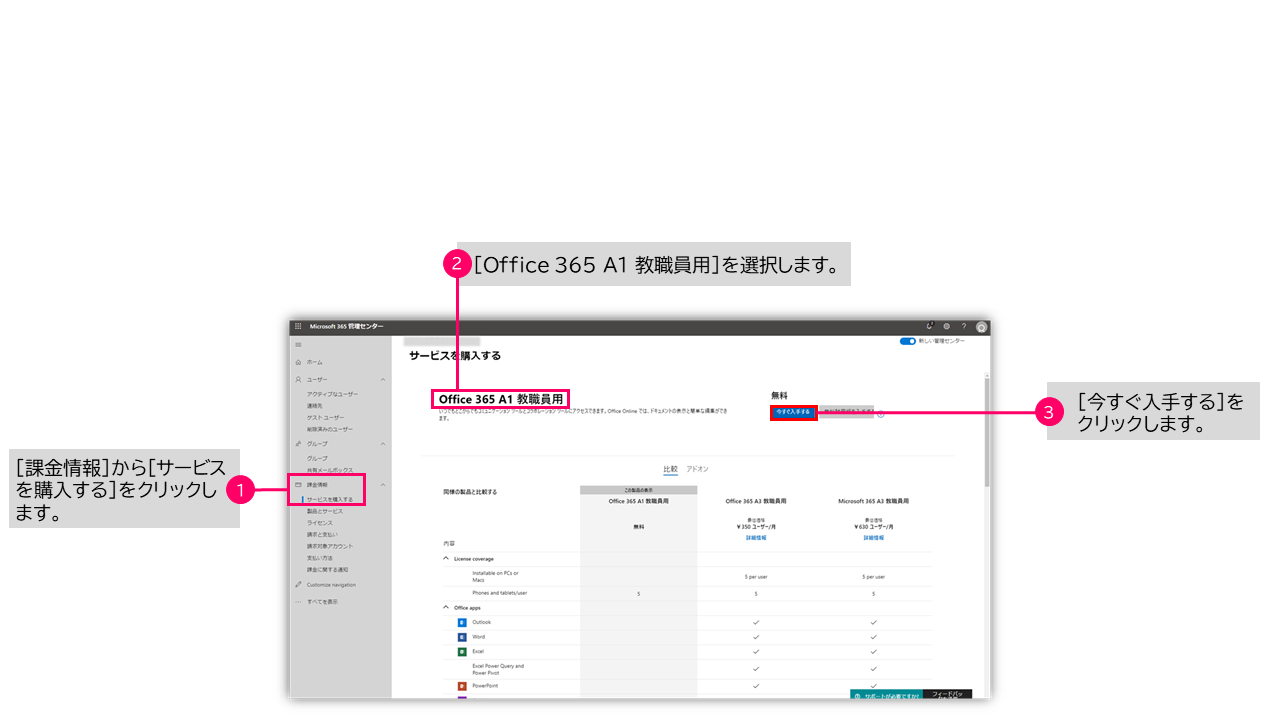
\includegraphics[width=10cm]{figures/O365A1_buy00.png}
    \end{minipage}
    \begin{minipage}{0.4\textwidth}
       Microsoft 365管理センターにグローバル管理者権限を持つユーザーでアクセスします。\\
       画面左のメニューから\textbf{【課金情報】→【サービスを購入する】}をクリックします。\\
       \textbf{【Office 365 A1 教職員用】}を選択します。\\
       \textbf{【今すぐ入手する】}をクリックします。
    \end{minipage}
\end{figure*}

\begin{figure*}[h]
    \begin{minipage}{0.6\textwidth}
        \vspace{-1.5cm}
        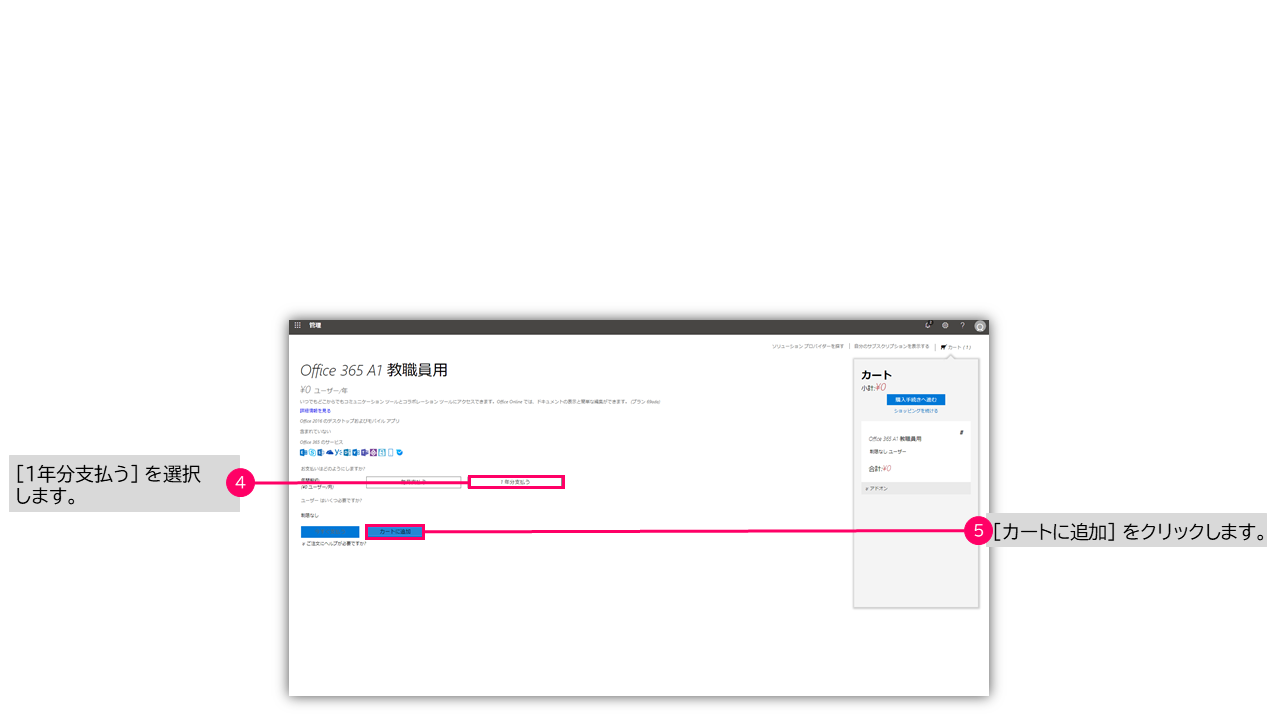
\includegraphics[width=10cm]{figures/O365A1_buy01.png}
    \end{minipage}
    \begin{minipage}{0.4\textwidth}
        \textbf{【毎月支払う】}または\textbf{【1年分支払う】}を選択します。\\
        \textbf{【カートに追加】}を選択します。
    \end{minipage}
\end{figure*}

\begin{figure*}[h]
    \begin{minipage}{0.6\textwidth}
        \vspace{-1.4cm}
        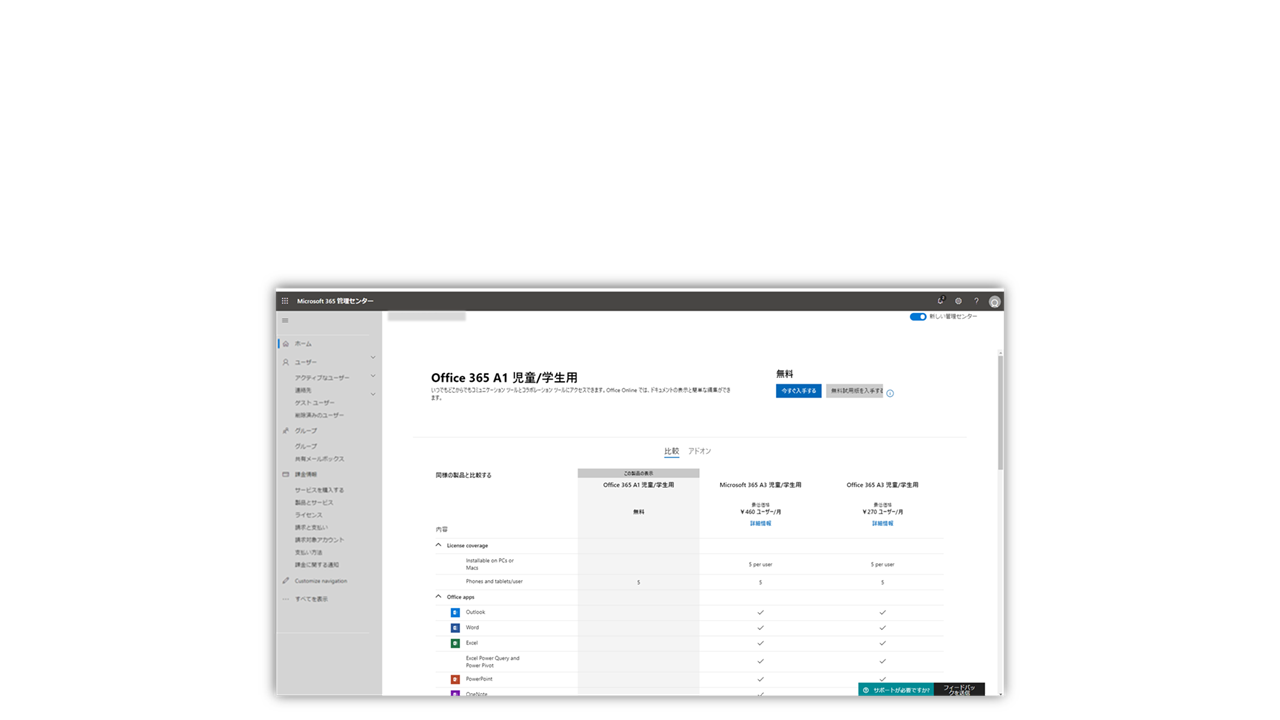
\includegraphics[width=10cm]{figures/O365A1_buy02.png}
    \end{minipage}
    \begin{minipage}{0.4\textwidth}
        児童/生徒用のライセンスも同様の手順でカートに追加します。
    \end{minipage}
\end{figure*}

\begin{figure*}[h]
    \begin{minipage}{0.6\textwidth}
        \vspace{-1.8cm}\hspace{-0.6cm}
        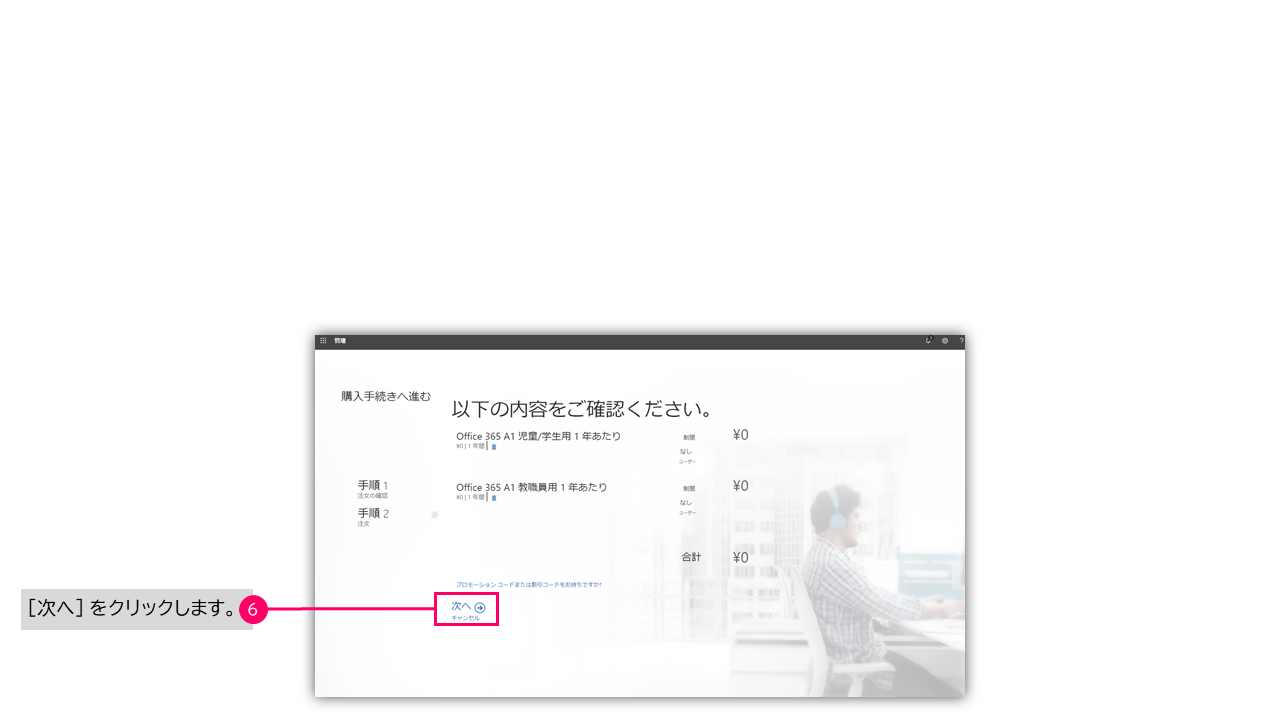
\includegraphics[width=11cm]{figures/O365A1_buy03.png}
    \end{minipage}
    \begin{minipage}{0.4\textwidth}
        カートのに登録された内容を確認し、問題ないようであれば\textbf{【次へ]}をクリックします。
    \end{minipage}
\end{figure*}

\begin{figure*}[h]
    \begin{minipage}{0.6\textwidth}
        \vspace{-2cm}\hspace{-0.8cm}
        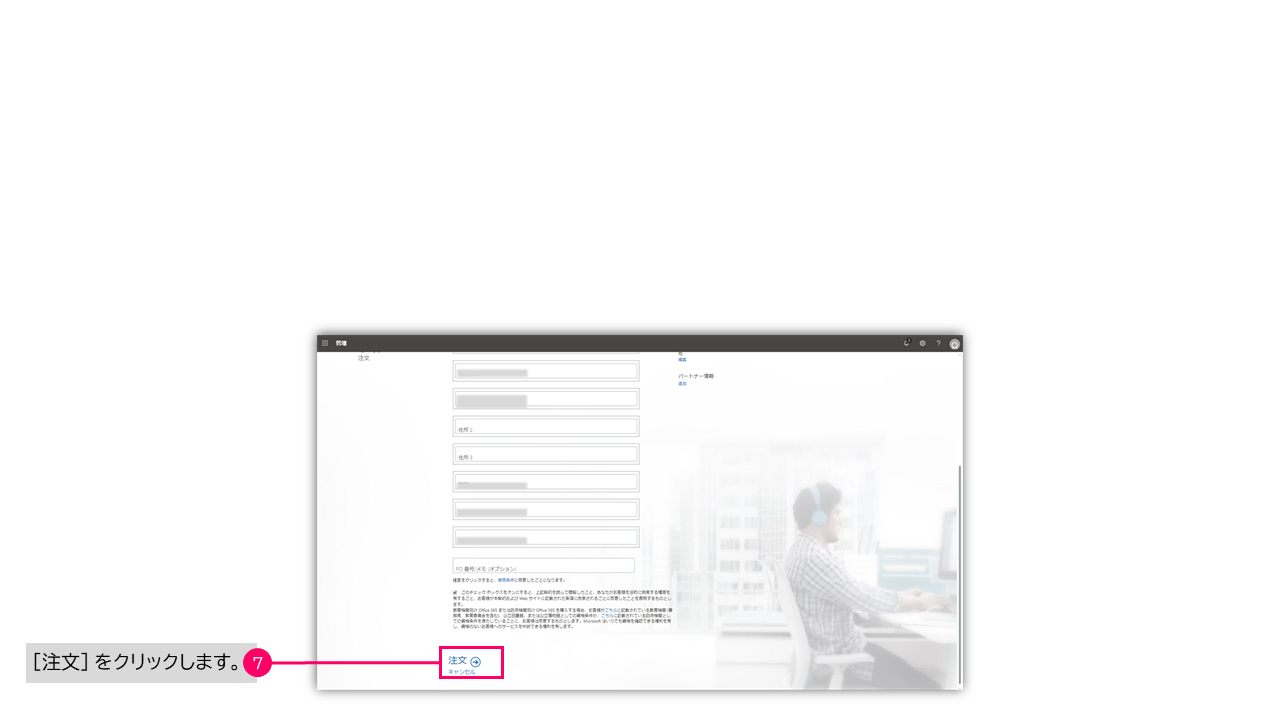
\includegraphics[width=11.5cm]{figures/O365A1_buy04.png}
    \end{minipage}
    \begin{minipage}{0.4\textwidth}
        最後に\textbf{【注文】}をクリックします。
    \end{minipage}
\end{figure*}

\begin{figure*}[h]
    \begin{minipage}{0.6\textwidth}
        \vspace{-2cm}
        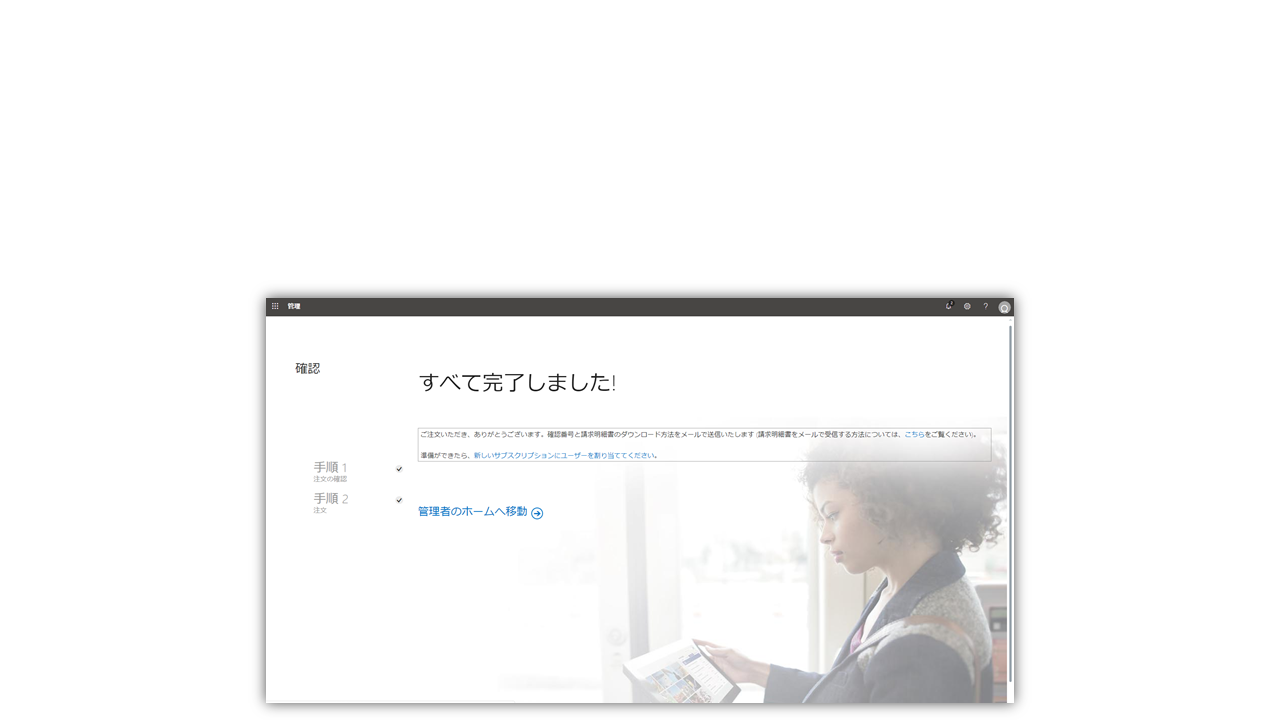
\includegraphics[width=10cm]{figures/O365A1_buy05.png}
    \end{minipage}
    \begin{minipage}{0.4\textwidth}
        これで Office 365 Education A1 の購入手続きは完了です。
    \end{minipage}
    \vspace{13cm}
\end{figure*}

